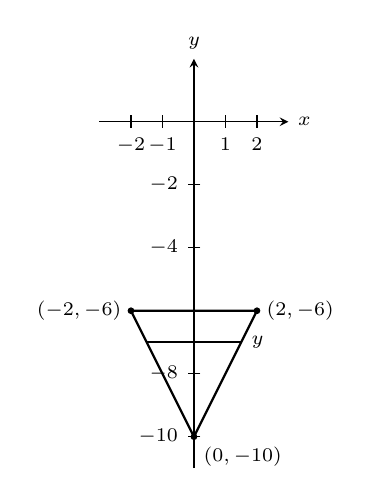
\begin{tikzpicture}[x=.4cm,y=.4cm,>=stealth]
\draw[thick] (0,0) -- (2,4) --  (-2,4) -- cycle;

\draw [fill=black] 	(2,4) circle (1pt) node [right] {\scriptsize $(2,-6)$}
										(-2,4)circle (1pt) node [left] {\scriptsize $(-2,-6)$}
										(0,0)circle (1pt) node [below right] {\scriptsize $(0,-10)$};
										
\draw [{\colortwo},thick]  (-1.5,3) -- (1.5,3) node [right,black] {\scriptsize $y$};
										
\draw [->] (0,-1) -- (0,12) node [above] {\scriptsize $y$};
\draw [->] (-3,10) -- (3,10) node [right] {\scriptsize $x$};

\foreach \x in {-2,-1,1,2}
{
	\draw (\x,10.2) -- (\x,9.8) node [below] {\scriptsize $\x$};
}

\foreach \x in {-10,-8,-4,-2}
{
	\draw (.2,{\x+10}) -- (-.2,{\x+10}) node [left] {\scriptsize $\x$};
}

\end{tikzpicture}

